\documentclass[12pt]{article} 
\usepackage{fullpage} 
\usepackage[affil-it]{authblk} 
\newcommand{\tab}{\hspace*{2em}}
\usepackage{graphicx} 
\graphicspath{ {.} } 
\usepackage{float} 
\usepackage{url} 
\usepackage{mhchem}
\usepackage{siunitx}

\begin{document} 

\title{Designing neutron shielding for a CENNS experiment} 

\author[1]{Jan P. Adam} 
\author[2]{Kate Scholberg} 
\affil[1]{Technische Universit\"at Dortmund, Fakult\"at Physik, Dortmund, Germany} 
\affil[2]{Duke University, Department of Physics, Durham, NC 27705} 
\date{October 4, 2014} 

\maketitle
\begin{abstract}
The Spallation Neutron Source (SNS) at Oak Ridge National Laboratory is also a neutrino source.  These particular neutrinos provide an optimal opportunity for the observation of coherent elastic neutrino-nucleus scattering (CENNS), a process that has been predicted but never observed. The detector configuration must involve some lead shielding surrounding the CENNS detector to block background radiation. However, the neutrinos must pass through this lead shielding to reach the detector, and doing so may produce neutrino-induced neutrons that can enter the detector and create a false signal. The Geant4 simulation toolkit was used to study neutron shielding and the neutron energy deposition in the detector volume.
\end{abstract}
\newpage

\section{Introduction}



\section{Simulation set up}

The Geant4 simulation toolkit was used to reproduce the results of. The detector set up can be seen in figure \ref{}. The detector's core consists of a lead cube (\SI{50}{cm} edge-length) with 4 holes that hold one EJ-301 scintillator, each. These are frustums of a cone and are made of pure liquid EJ-301 (\cf{C_8H_{10}}). The sides and the bottom of the lead cube are covered with a \SI{1}{cm} thick layer of EJ-200 a solid plastic scintillator (\cf{C_{10}H_{11}}]). Above the lead cube is a gap of \SI{21}{cm} followed by an Al-7075 plate with a thickness of \SI{2}{cm}. This plate shall reduce signals of cosmic neutrinos in the real detector. The whole setup is enclosed by a \SI{1}{m^3} water cube.

Neutrons are being generated randomly inside the lead with a random direction.

If a particle enters one of the scintillators and deposits energy, that amount will be converted into electron-equivalent energy by using the graph in figure \ref{fig:photonResponse}.

\begin{figure}[htbp]
	\centering
	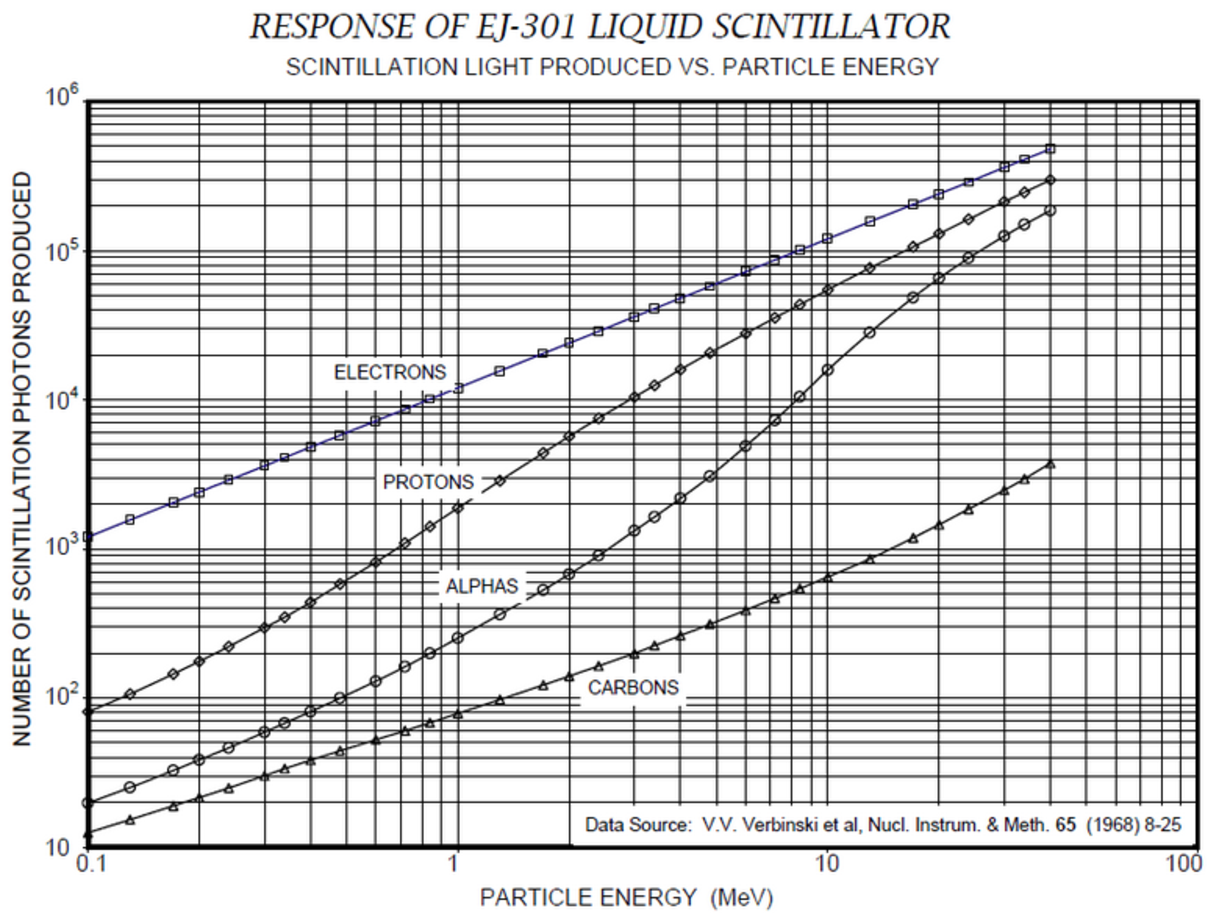
\includegraphics[width=0.7\textwidth]{./pics/scintillatorResponse.pdf}
	\caption{Photon response of the EJ-301 scintillator.}
	\label{fig:photonResponse}
\end{figure}
In addition to the four particles mentioned in this graph there is also a number of $\gamma$, $e^+$ and deuterons that enter the scintillator. Since $e^+$ have the same mass and charge as electrons and $\gamma$ will decay into $e^- + e^+$ both of them are treated as electrons. Deuterons will approximately emit a number of photons that lies in the middle between $p$ and $\alpha$. In approx. 0.5\% of the events the reaction \ce{n^1_0 + C^{12}_6 -> C^{13}_6 -> B^9_4 + \alpha^4_2 } can occur. In this case the electron-equivalent energy of the beryllium nucleus will not be calculated. This effect should be negligible, though.

\section{Results and Discussion}

\subsection{Correct set up}

First of all, it was necessary to verify that the neutrons were generated in the correct volume. Figure \ref{} and \ref{} show that the particles were generated only inside the lead and not inside the holes which contain the scintillators. Figure \ref{} and \ref{} show that the direction of the neutrons is equally distributed.

\subsection{Efficiency}

An event will be marked as "valid" once the energy deposition in a single scintillator exceeds a given threshold in keVee. It is also noted if multiple scintillators received "valid" signals in a single event. Figure \ref{} and \ref{} show the percentage of events which were marked as "valid" at a given energy of the primary particle with an energy threshold of \SI{30}{keVee} and \SI{100}{keVee}. Figure \ref{} and \ref{} show the results of the MCNP simulation.







\section{Conclusion}


\section*{Acknowledgments}
\begin{itemize}
  \item[] Kate Scholberg and the Duke Neutrino Group.
\end{itemize}

\bibliographystyle{my_utphys}
\bibliography{Final}

\end{document}
